\panel{\begin{tikzpicture}[x=1bp, y=1bp]\path[use as bounding box] (0,0) rectangle (132.60,115.80);\clip (0,0) rectangle (132.60,115.80);
\path[fill={rgb,255:red,220;green,252;blue,231}] (7.50,57.90) rectangle (87.30,108.30);
\path[fill={rgb,255:red,219;green,234;blue,254}] (7.50,7.50) rectangle (87.30,57.90);
\path[draw={rgb,255:red,71;green,85;blue,105}, line width=1.20bp, dash pattern=on 3.75bp off 3.00bp, line cap=round, line join=round] (7.50,57.90) -- (87.30,57.90);
\path[draw={rgb,255:red,30;green,58;blue,138}, line width=2.25bp, line cap=round, line join=round] (87.30,7.50) -- (87.30,108.30);
\node[anchor=base west, text={rgb,255:red,30;green,58;blue,138}, font=\fontsize{8.2}{9.9}\selectfont\sffamily, inner sep=0pt] at (91.80,97.80) {wall x = 1};
\path[draw={rgb,255:red,220;green,38;blue,38}, line width=1.65bp, -{Triangle[length=9.2bp, width=9.2bp]}, line cap=round, line join=round] (53.70,91.50) -- (86.04,59.16);
\path[draw={rgb,255:red,71;green,85;blue,105}, line width=1.35bp, fill=white] (87.30,57.90) circle[radius=3.00bp];
\node[anchor=base west, text={rgb,255:red,71;green,85;blue,105}, font=\fontsize{8.2}{9.9}\selectfont\sffamily, inner sep=0pt] at (92.55,54.90) {E2};
\node[anchor=base west, text={rgb,255:red,21;green,128;blue,61}, font=\fontsize{9.0}{10.8}\selectfont\sffamily\bfseries, inner sep=0pt] at (20.10,83.10) {P1};
\node[anchor=base west, text={rgb,255:red,29;green,78;blue,216}, font=\fontsize{9.0}{10.8}\selectfont\sffamily\bfseries, inner sep=0pt] at (20.10,32.70) {P0};
\end{tikzpicture}}{(a) In your room}\hspace{22.5bp}\panel{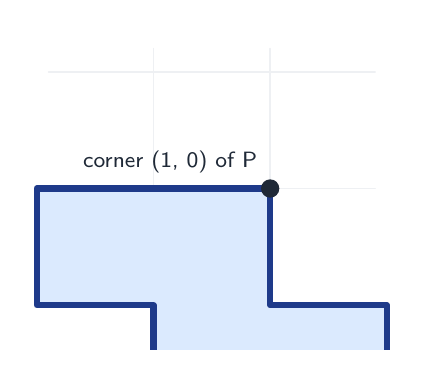
\begin{tikzpicture}[x=1bp, y=1bp]\path[use as bounding box] (0,0) rectangle (132.60,115.80);\clip (0,0) rectangle (132.60,115.80);
\path[draw={rgb,255:red,238;green,240;blue,243}, line width=0.52bp, line cap=round, line join=round] (45.30,7.50) -- (45.30,108.30);
\path[draw={rgb,255:red,238;green,240;blue,243}, line width=0.52bp, line cap=round, line join=round] (87.30,7.50) -- (87.30,108.30);
\path[draw={rgb,255:red,238;green,240;blue,243}, line width=0.52bp, line cap=round, line join=round] (7.50,15.90) -- (125.10,15.90);
\path[draw={rgb,255:red,238;green,240;blue,243}, line width=0.52bp, line cap=round, line join=round] (7.50,57.90) -- (125.10,57.90);
\path[draw={rgb,255:red,238;green,240;blue,243}, line width=0.52bp, line cap=round, line join=round] (7.50,99.90) -- (125.10,99.90);
\path[draw={rgb,255:red,30;green,58;blue,138}, line width=2.25bp, fill={rgb,255:red,219;green,234;blue,254}, line join=round] (3.30,57.90) -- (87.30,57.90) -- (87.30,15.90) -- (129.30,15.90) -- (129.30,-68.10) -- (87.30,-68.10) -- (87.30,-26.10) -- (45.30,-26.10) -- (45.30,15.90) -- (3.30,15.90) -- cycle;
\path[fill={rgb,255:red,31;green,41;blue,55}] (87.30,57.90) circle[radius=3.30bp];
\node[anchor=base east, text={rgb,255:red,31;green,41;blue,55}, font=\fontsize{8.2}{9.9}\selectfont\sffamily, inner sep=0pt] at (82.80,65.40) {corner (1, 0) of P};
\end{tikzpicture}}{(b) Folded into $P$: draw both directions here}
